
                \begin{figure}
                    \centering
                    \begin{tikzpicture}
                        \pgfplotsset{%
                            width=1\textwidth,
                            height=0.4\textheight
                        }
                        \begin{axis}[
                            xlabel={Runs since restart},
                            ylabel={Average dynamic energy (watt)},
                            ymin=0,ymax=70,
                        ]
                        
                            \addplot [mark=none, densely dashed, red]  coordinates {
                            (1, 29.31988512605307)(2, 28.472409388936953)(3, 28.647417166957183)(4, 28.536463089627745)(5, 28.589476892982386)
                            };
                            \addlegendentry{WRK - IPG}
                            
                            \addplot [mark=none, densely dashed, blue]  coordinates {
                            (1, 30.841462981069082)(2, 28.745834086118098)(3, 28.350271131322664)(4, 28.75859151425193)(5, 28.286696336648827)
                            };
                            \addlegendentry{WRK - LHM}
                            
                            \addplot [mark=none, densely dashed, cyan]  coordinates {
                            (1, 16.671237185180534)(2, 25.804294689797715)(3, 19.46855807922392)(4, 17.68514444673619)(5, 26.65591249329199)
                            };
                            \addlegendentry{WRK - CLAMP (win)}
                            
                        \end{axis}
                    \end{tikzpicture} 
                \caption{A graph illustrating the energy consumption of Cores for test case Fasta with regards to how long ago the DUT was restarted, experiment \#2, (with outliers)} \label{fig:Fasta_Cores_iteration_exp2}
                \end{figure}
                